\documentclass{article}
\usepackage{tikz}      
\usetikzlibrary{calc}  

\newcount\depth

\makeatletter
\newcommand*\bernoulliTree[1]{%
    \depth=#1\relax            
    \draw node(root)[bernoulli/root] {}[grow=down] \draw@bernoulli@tree;
    \draw \label@bernoulli@tree{root};                                   
}                                                                        

\def\draw@bernoulli@tree{%
    \ifnum\depth>0        
      child foreach \type/\label in {left child/$S$,right child/$F$} {%
          node[bernoulli/\type]{\label} \draw@bernoulli@tree
      }
      coordinate[bernoulli/increment] (dummy)
   \fi%
}

\def\label@bernoulli@tree#1{%
    \ifnum\depth>0        
      child foreach \type/\label in {left child/$S$,right child/$F$} {%
          node[bernoulli/\type]{\label} \draw@bernoulli@tree
      }
      coordinate[bernoulli/increment] (dummy)
   \fi%
}

\makeatother

\tikzset{bernoulli/.cd,
         root/.style={draw,rectangle},
         decrement/.code=\global\advance\depth by-1\relax,
         increment/.code=\global\advance\depth by 1\relax,
         left child/.style={draw,bernoulli/decrement},
         right child/.style={draw,rectangle}}

\begin{document}
%\resizebox{\linewidth}{!}{%
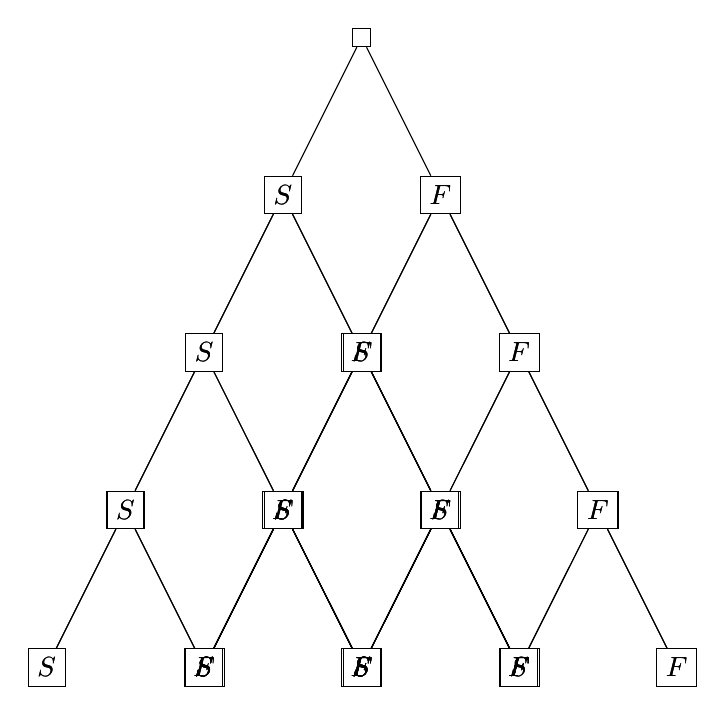
\begin{tikzpicture}[level distance=2cm,
                    level 1/.style={sibling distance=2cm},
                    level 2/.style={sibling distance=2cm},
                    level 3/.style={sibling distance=2cm},
                    level 4/.style={sibling distance=2cm},
                    level 5/.style={sibling distance=2cm},
                    level 6/.style={sibling distance=2cm}]
\bernoulliTree{4}
\end{tikzpicture}
%}
\end{document}